\documentclass{article}
\usepackage[UTF8]{ctex}  % 使用中文支持包
\usepackage[a4paper, margin=1in]{geometry}  % 设置纸张大小和边距
\usepackage{anyfontsize}  % 解决字体大小报错问题
\usepackage{fancyhdr}  % 设置页眉、页脚、页码
\usepackage{longtable}  % 支持长表格

\usepackage{amsmath}  % 数学公式支持
\usepackage{cases}  % 支持联立编号
\usepackage{cite}  % 引用支持

\usepackage{graphicx}  % 插入图片支持
\usepackage{float}  % 设置图片浮动位置
\usepackage{subfigure}  % 插入多图时用子图显示

\usepackage{listings}  % 代码块支持
\usepackage{xcolor}  % 设置代码块颜色

\usepackage[hyphens]{url}  % 支持链接换行
\usepackage{hyperref}  % 超链接支持
\usepackage{lastpage}  % 添加lastpage包

\usepackage{gbt7714}  %国标参考文献

\hypersetup{
    hidelinks,
    colorlinks=true,
    allcolors=black,
    pdfstartview=Fit,
    breaklinks=true
}

\title{聚变能源概论-第六讲作业}
\author{\LaTeX\ by\ Jerry\ }
\date{\today}
\pagenumbering{arabic}

\begin{document}
\pagestyle{fancy}

\fancyhead[L]{Jerry}
\fancyhead[C]{聚变能源概论-第六讲作业}
\fancyhead[R]{\today}
\fancyfoot[C]{Page \thepage/\pageref{LastPage}}

\section*{5.1}

\emph{在一幅对数-对数坐标的 $n_e-T_e$ 图上绘制出 $\lambda _D$ 和 $N_D$ 的等值线,$n_e$ 范围为 $10^6\sim10^{25}m^{-3}$,$T_e$ 范围为 $10^{-2}\sim10^5eV$。然后,在这张图上标出以下点:
\begin{itemize}
    \item 典型的聚变反应堆: $n_e=10^{21}, T_e=10^4$
    \item 典型的聚变实验: $n_e=10^{19}, T_e=10^2$ (环);$n_e=10^{23}, T_e=10^3$(箍缩)
    \item 典型的电离层: $n_e=10^{11}, T_e=0.05$
    \item 典型的辉光放电: $n_e=10^{14}, T_e=2$
    \item 典型的火焰: $n_e=10^{14}, T_e=0.1$
    \item 典型的绝等离子体: $n_e=10^{17}, T_e=0.2$
    \item 星际空间: $n_e=10^6, T_e=0.01$
\end{itemize}}

$$\lambda_D = \sqrt{\frac{\varepsilon_0 T_e}{n_e e^2}} \Rightarrow n_e = \frac{\varepsilon_0 T_e}{\lambda_D^2 e^2}$$

$$N_D = n\lambda_D^3 = n_e \left( \frac{\varepsilon_0 T_e}{n_e e^2} \right)^{3/2} \Rightarrow n_e = \frac{1}{N_D^{2/3}} \left( \frac{\varepsilon_0 T_e}{e^2} \right)^{3/2} = \frac{\varepsilon_0^{3/2}T_e^{3/2}}{N_D^{2/3}e^6}$$

故$\lambda_D$ 等值线为 $$\lg(n_e) = \lg(T_e) + \lg\left(\frac{\varepsilon_0}{\lambda_D^2 e^2}\right)$$

$N_D$ 等值线为 $$\lg(n_e) = 3\lg(T_e) + \lg\left(\frac{\varepsilon_0^{3/2}}{N_D^{2/3}e^6}\right)$$

$\lg(n)-\lg(T_e)$ 关系图如\ref{fig:1},蓝色、橙色虚线分别代表德拜长度$\lambda_D$、等离子体参数$N_D$等值线

\begin{figure}[htbp]
    \centering
    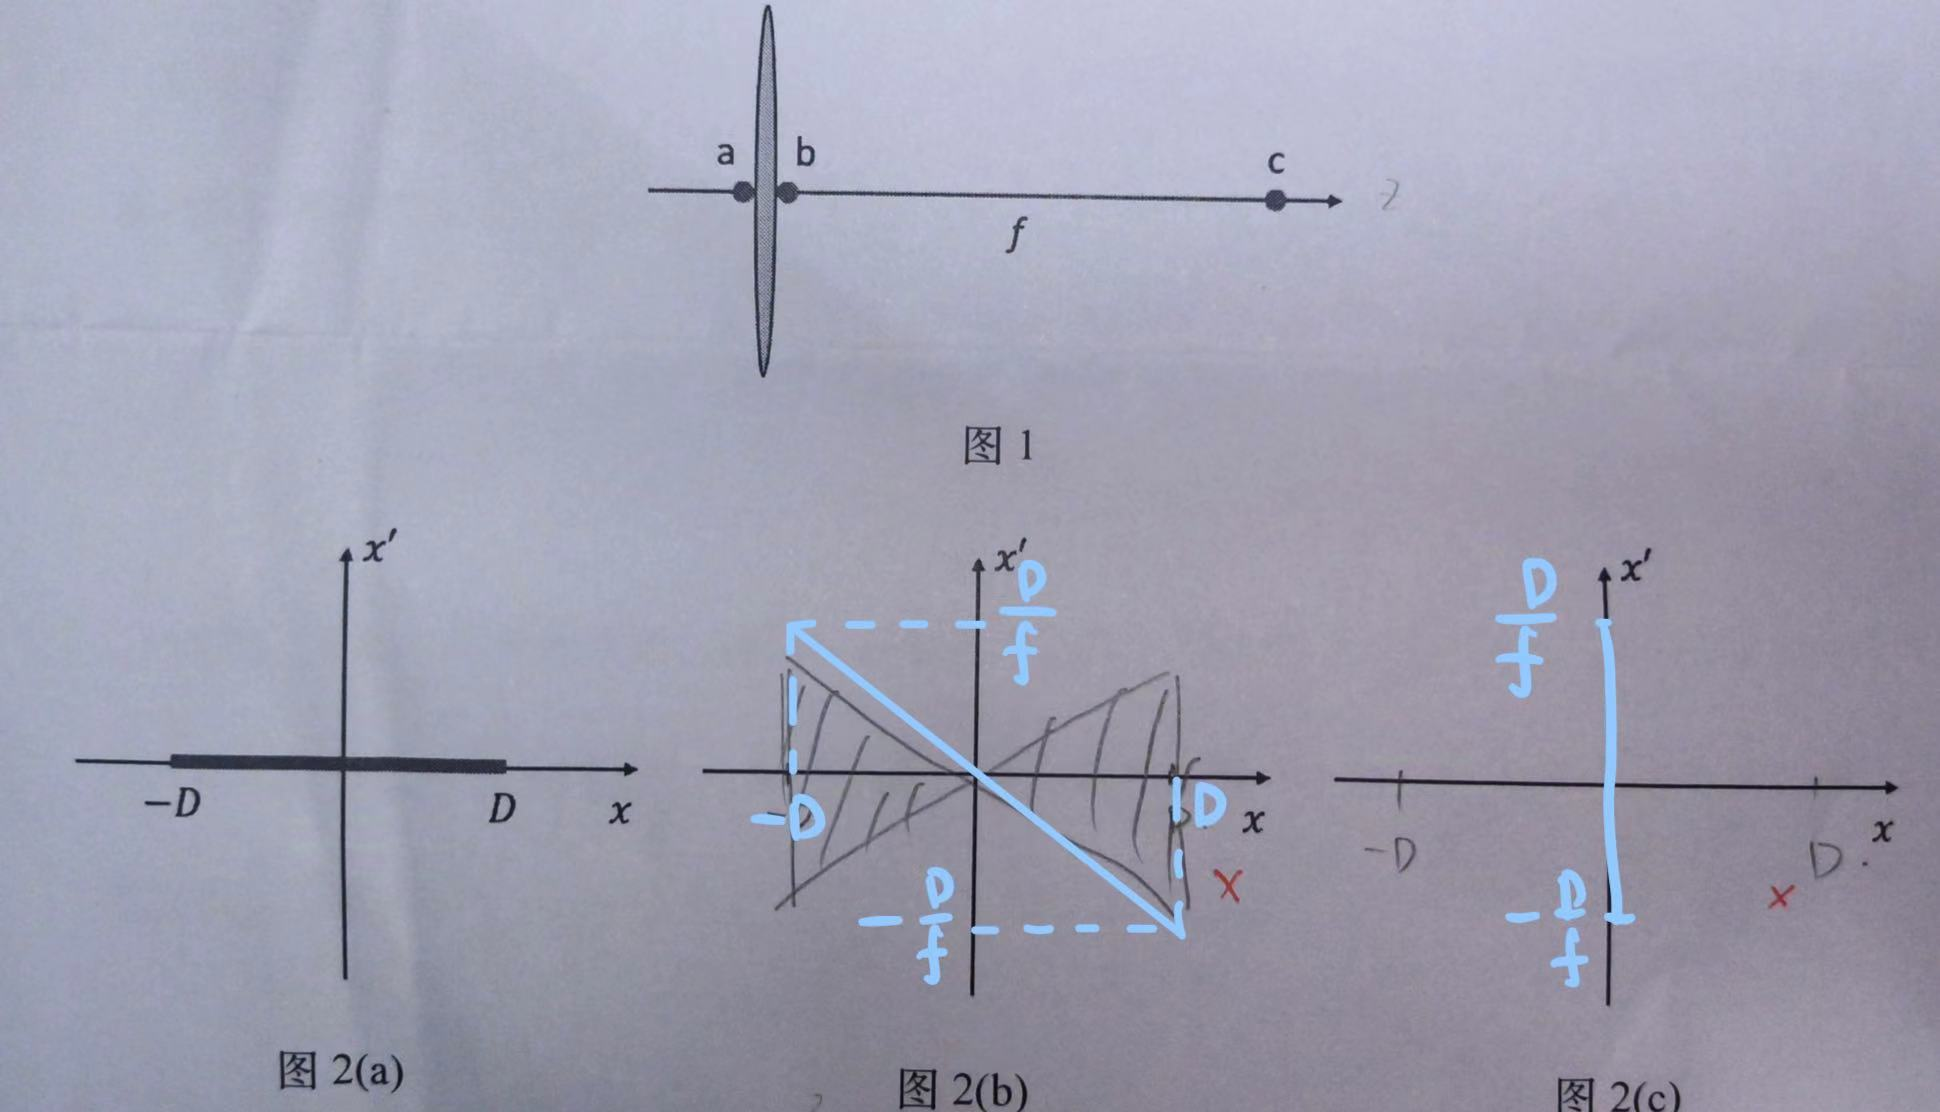
\includegraphics[width=0.6\textwidth]{img/1.pdf}
    \caption{$\lg(n)-\lg(T_e)$ 关系图}
    \label{fig:1}
\end{figure}

\section*{5.2}

\emph{证明磁矩在变化远慢于回旋频率的缓变磁场中是个浸渐不变量。(提示:见本章参考书[1])}

磁矩是一个绝热不变量,即粒子在磁力线上来回跑时,磁矩不变,故有$$\frac{\partial \mu}{\partial s} = 0 $$

等价于证明 $$F_{z} = - \mu \frac{\partial B}{\partial s}$$

设磁场主要沿着z方向且无角向分量,并在z方向上有着缓慢的变化,以认为$B_z$方向的分量占主导并近似平行方向为z方向,要证明的式子变为$$F_{z}=-\mu \frac{\partial B}{\partial s}\approx -\mu \frac{\partial B_{z}}{\partial z}$$

而洛伦兹力给出的表达式是$$ F_{z} =-qv_{\theta }B_{r} $$

又有$$\nabla \cdot B=0 $$将$B_{r} $与$B_{z} $联系起来就可以了。磁场线守恒$\nabla \cdot B=0$在柱坐标系展开为$$\frac{1}{r}\frac{\partial }{\partial r}(rB_{r})+\frac{\partial B_{z}}{\partial z}=0$$
利用缓变条件,设$\frac{\partial B_{z}}{\partial z} $与$r$不相关,直接积分就可得到
\begin{equation*}
    \begin{aligned}
        (r'B_{r})\bigg|_{r'=0} &= -\frac{\partial B_{z}}{\partial z} \int_{0}^{r'} r' \mathrm{d}r' = -\frac{1}{2} r^2 \frac{\partial B_{z}}{\partial z} \\
        B_{r} &= -\frac{r}{2} \frac{\partial B_{z}}{\partial z}
    \end{aligned}
\end{equation*}

代回$F_{z} =-qv_{\theta }B_{r} $,得到

\begin{equation*}
    \begin{aligned}
        F_{z} &= qv_{\theta }\frac{r}{2}\frac{\partial B_{z}}{\partial z} \\
        &= \frac{1}{2} qv_{\theta }\frac{mv_{\theta }}{qB_{z} }\frac{\partial B_{z}}{\partial z} \\
        &= \frac{1}{2} mv_{\theta }^{2}\frac{\partial B_{z}}{\partial z} \\
        &= -\mu  \frac{\partial B_{z}}{\partial z}
    \end{aligned}
\end{equation*}

故磁矩是一个浸渐不变量。

\end{document}
